\documentclass[]{article}
\usepackage{hyperref}
\hypersetup{
    colorlinks=true,
    linkcolor=blue,
    filecolor=magenta,      
    urlcolor=blue,
}
\usepackage{graphicx}
\graphicspath{ {./images/} }

\begin{document}

	\title{Wifiology Final Submission}
	\author{
	Robert Cope, Jason Nguyen, Baiyu Chen,  \\
	Jasper Niemeyer, Peng Jiang, Ryan Campbell\\
	Group: 404 Group Not Found (104-2)}
	\maketitle

	\section{Process Tools}
	\subsection{Progress Tracking -- Trello}
	\paragraph{} For this project we used Trello for making and using Kanban cards to track progress. Our Trello board is located 
	at \href{https://trello.com/b/VvROa8e0/wifiology}{https://trello.com/b/VvROa8e0/wifiology.} It is currently set to private, but
	we plan to set this to public in the very near future. If you are unable to access this board, please reach out to Robert Cope
	(roco9727@colorado.edu) and Jasper Niemeyer (jani5714@colorado.edu) to request access. An image of our Trello board is shown in
	figure \ref{fig:trello_board}.
		
	\begin{figure}[h]
	\label{fig:trello_board}
	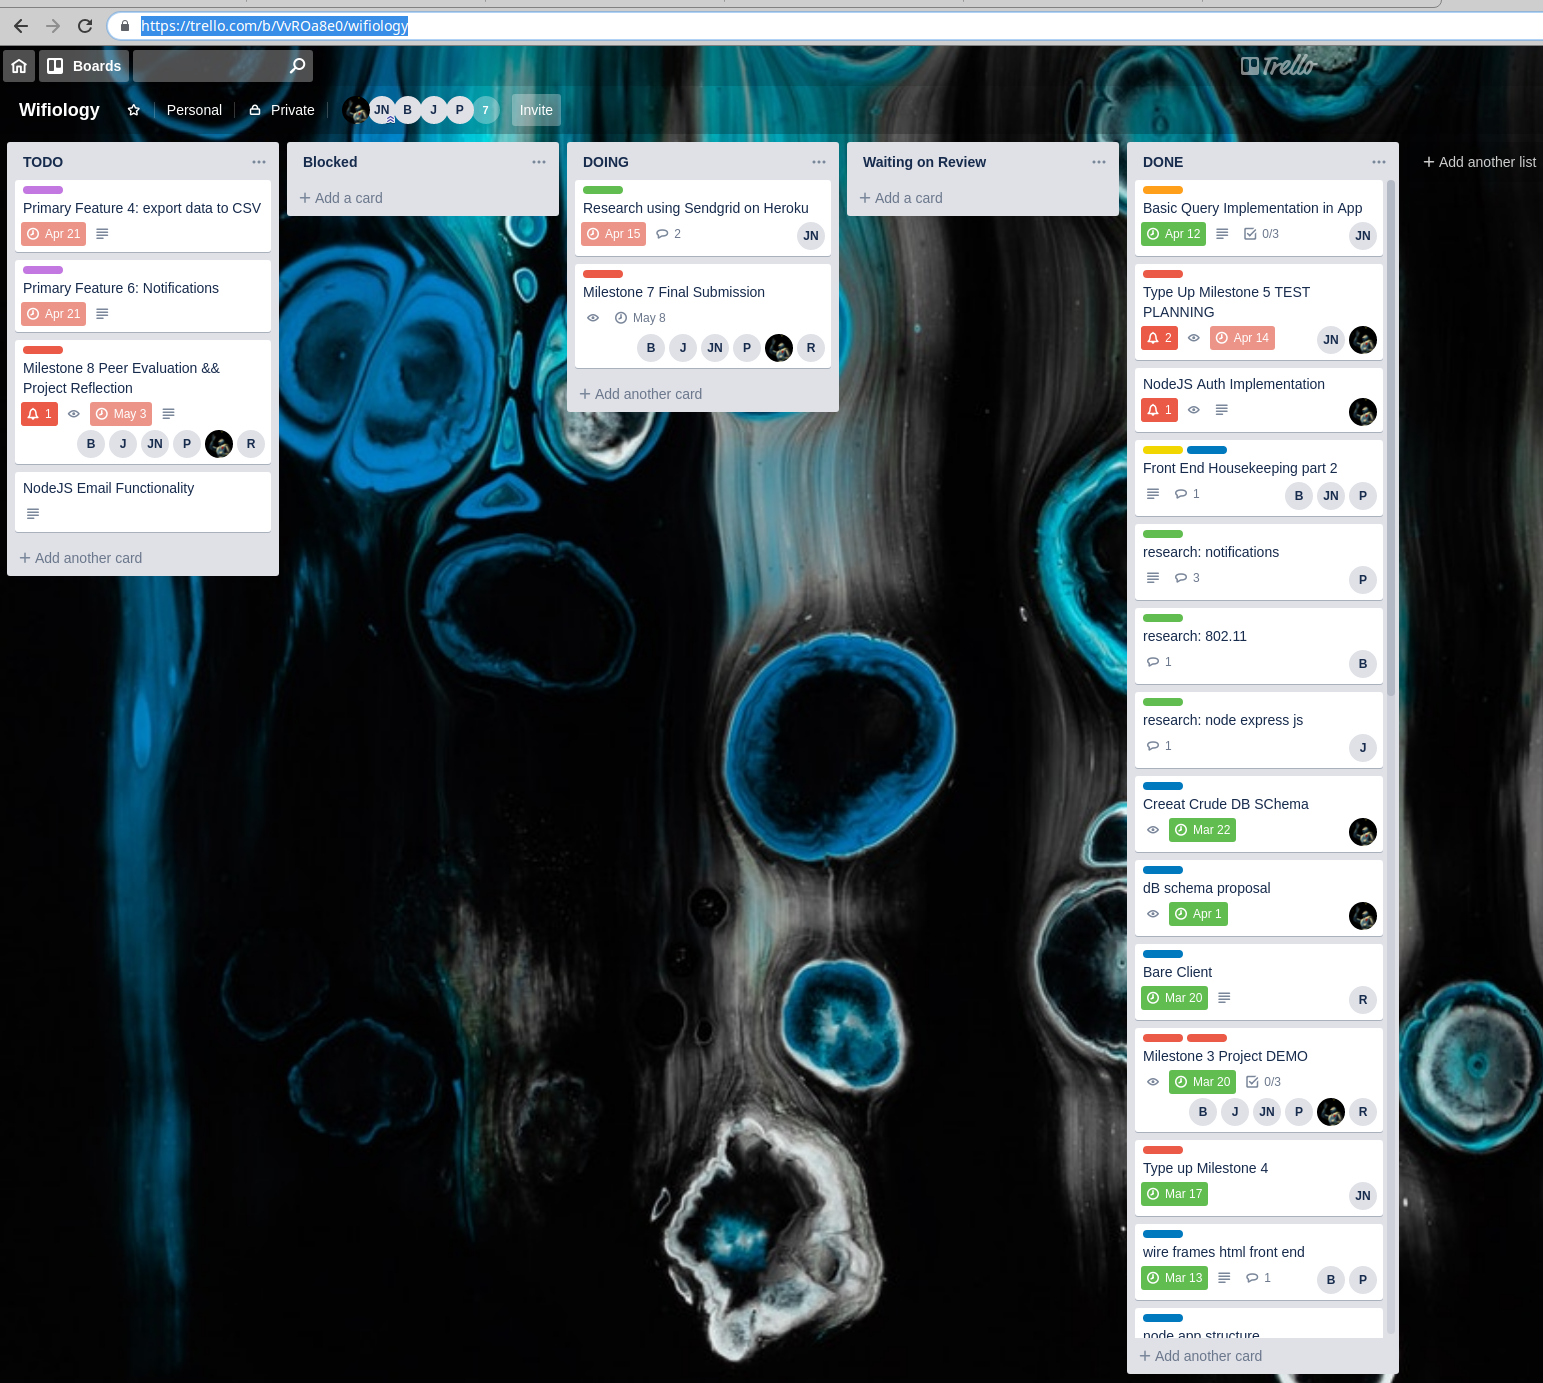
\includegraphics[width=1.0\textwidth]{trello}
	\caption{Wifiology Trello Board}
	\end{figure}

	\subsection{Version Control -- Git and Github}
	\paragraph{} For this project all of our code is stored on public repositories in Github under the 404 Group Not Found
	Github group, located at \href{https://github.com/404-group-does-not-exist}{https://github.com/404-group-does-not-exist}.
	The project is constituted of several repositories. Our milestones may be found at \href{https://github.com/404-group-does-not-exist/milestones}{https://github.com/404-group-does-not-exist/milestones}, and our minutes may be found at 
	\href{https://github.com/404-group-does-not-exist/minutes}{https://github.com/404-group-does-not-exist/minutes}. The source
	code for the NodeJS central server may be found at \href{https://github.com/404-group-does-not-exist/Wifiology}{https://github.com/404-group-does-not-exist/Wifiology}. The code for the listener node may be found at \href{https://github.com/404-group-does-not-exist/client\_proof\_of\_concept}{https://github.com/404-group-does-not-exist/client\_proof\_of\_concept}. The source code for our Android app
	may be found at \href{https://github.com/404-group-does-not-exist/wifiology\_android\_app}{https://github.com/404-group-does-not-exist/wifiology\_android\_app}, and the source code for our Selenium tests may be found at \href{https://github.com/404-group-does-not-exist/Selenium}{https://github.com/404-group-does-not-exist/Selenium}. Please node we have foregone using a monorepo for the codebase listed 
	above to ease development of separate concerns; for the sake of this final submission, we have chosen to keep the repositories 
	separate to allow graders a more honest look into commit history (rather than bringing everything into a single repository at the
	last moment, and potentially losing all commit history).
	
	\subsubsection{Structure}
	\paragraph{}
    It is important to understand the basic application architecture in order to understand the repository structure. The basic
    organization of the Wifiology ecosystem and architecture is given in figure \ref{fig:architecture}. There any many listener
    nodes, each potentially deployed and managed by separate users; the code for the listener nodes is contained completely in
    the repository at \href{https://github.com/404-group-does-not-exist/client\_proof\_of\_concept}{https://github.com/404-group-does-not-exist/client\_proof\_of\_concept}. The central server is deployed once, and is written in NodeJS; it can be found in its entirely in the
    repository at \href{https://github.com/404-group-does-not-exist/Wifiology}{https://github.com/404-group-does-not-exist/Wifiology}. 
    This repository also includes the web front-end for Wifiology.
    
    \paragraph{} The Android application also shown in the architecture diagram (figure \ref{fig:architecture}) is stored entirely in
    the repository located at \href{https://github.com/404-group-does-not-exist/wifiology\_android\_app}{https://github.com/404-group-does-not-exist/wifiology\_android\_app}.
	
	\begin{figure}[h]
	\label{fig:architecture}
	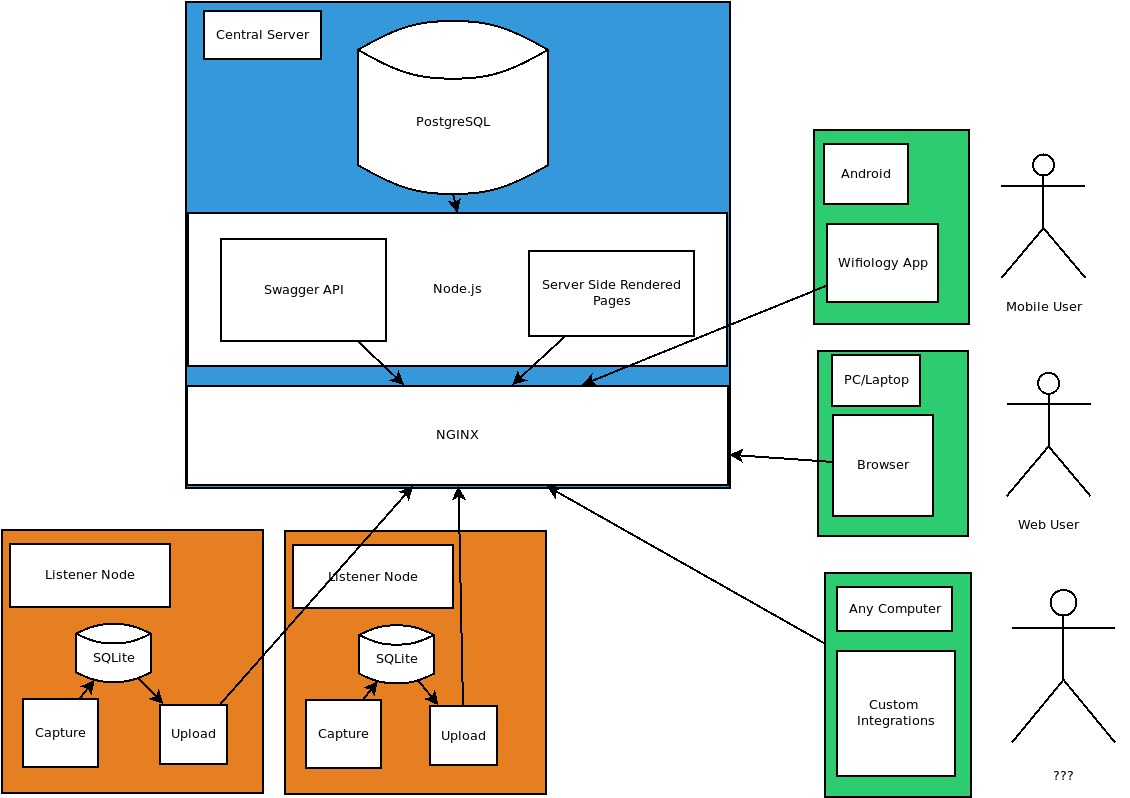
\includegraphics[width=1.0\textwidth]{basicWifiologyArchitecture}
	\caption{Wifiology Architecture}
	\end{figure}
	
	
	
	\subsubsection{Tests}
	
	\paragraph{} For the ``\texttt{client\_proof\_of\_concept}" repository, which is our listener node, 
	unit tests may be run by setting up a
	Python virtual environment, installing the requirements using \texttt{pip install -r requirements} and then using 
	\texttt{nose test\_wifiology\_node\_proof\_of\_concept} to run our unit tests.
	
	\paragraph{} For the ``\texttt{Wifiology}" repository, which is our central server, the tests may be run using
	\texttt{npm test}. Please note that the application and tests were designed to be run with the latest LTS version
	of NodeJS (which is 10.13.0); please ensure you have the version of NodeJS running (likely using the \texttt{nvm} 
	Node versioning tool to select it) prior to executing the tests.
	
	\paragraph{} The selenium tests may be run my cloning the selenium repository, ensuring the current instance of 
	Python has selenium webdriver installed, and then executing each script by giving it as the first argument to
	a new Python interpreter.
	
	\subsection{Continuous Integration}
	
	We utilized Travis CI for our continuous integration. Our Travis CI jobs can be seen at 
	\href{https://travis-ci.org/404-group-does-not-exist}{https://travis-ci.org/404-group-does-not-exist}.
	
	\subsection{Demo Video}
	
	A demo video of our web application can be found at \href{	https://f001.backblazeb2.com/file/rpc-public-bucket/vokoscreen-2019-05-05\_17-37-50.mkv}{https://f001.backblazeb2.com/file/rpc-public-bucket/vokoscreen-2019-05-05\_17-37-50.mkv}.
	
	\subsection{Individual Contributions}
	\subsubsection{Robert Cope}
	See the included code contribution figures. Robert contributed to the core Wifiology NodeJS application, the
	listener node, and to the operations and deployment for the project deployment.
	
	\subsubsection{Jason Nguyen}
	See the included code contribution figures. Jason contributed to the listener node codebase.	
	
	\subsubsection{Baiyu Chen}
    See the included code contribution figures. Baiyu contributed to the core Wifiology NodeJS application and the 
    Selenium tests.
	
	\subsubsection{Jasper Niemeyer}
    See the included code contribution figures. Jasper was also the project manager for our project and did much
    of our clerical work; Jasper also contributed to the core Wifiology NodeJS application and much of our operations work.
	
	\subsubsection{Peng Jiang}
    See the included code contribution figures. Pend contributed to the core Wifiology NodeJS application.
	
	\subsubsection{Ryan Campbell}
	See the included code contribution figures. Ryan contributed to the core Wifiology NodeJS application and
	the Android application.
	
	\begin{figure}[h]
	\label{fig:android_app_contrib}
	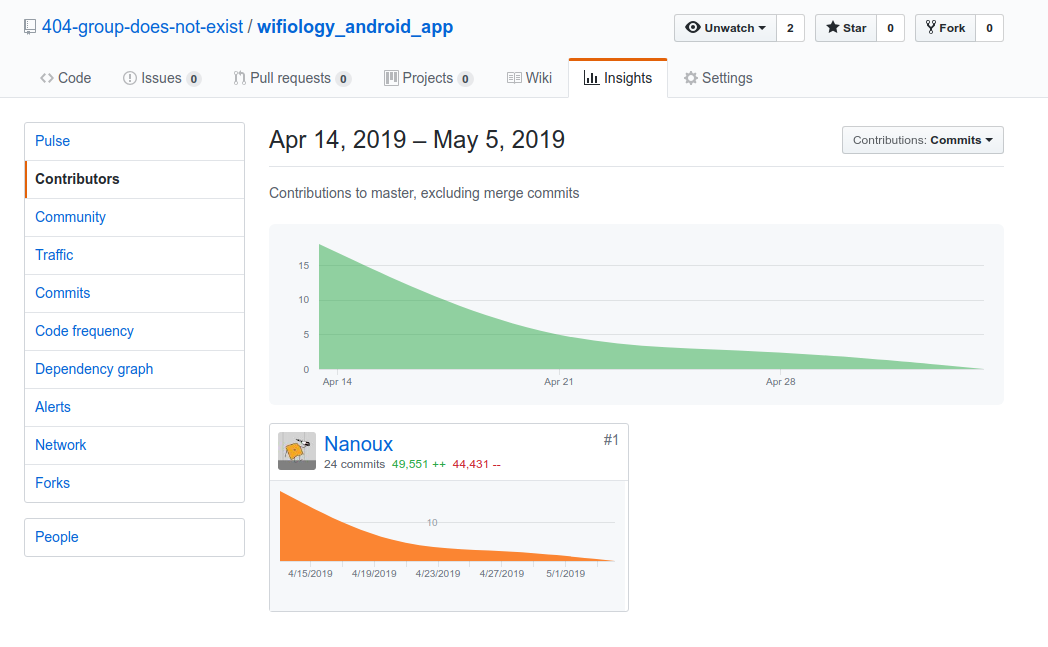
\includegraphics[width=1.0\textwidth]{androidAppContrib}
	\caption{Android App Contributions}
	\end{figure}
	
	\begin{figure}[h]
	\label{fig:wifiology_test_contrib}
	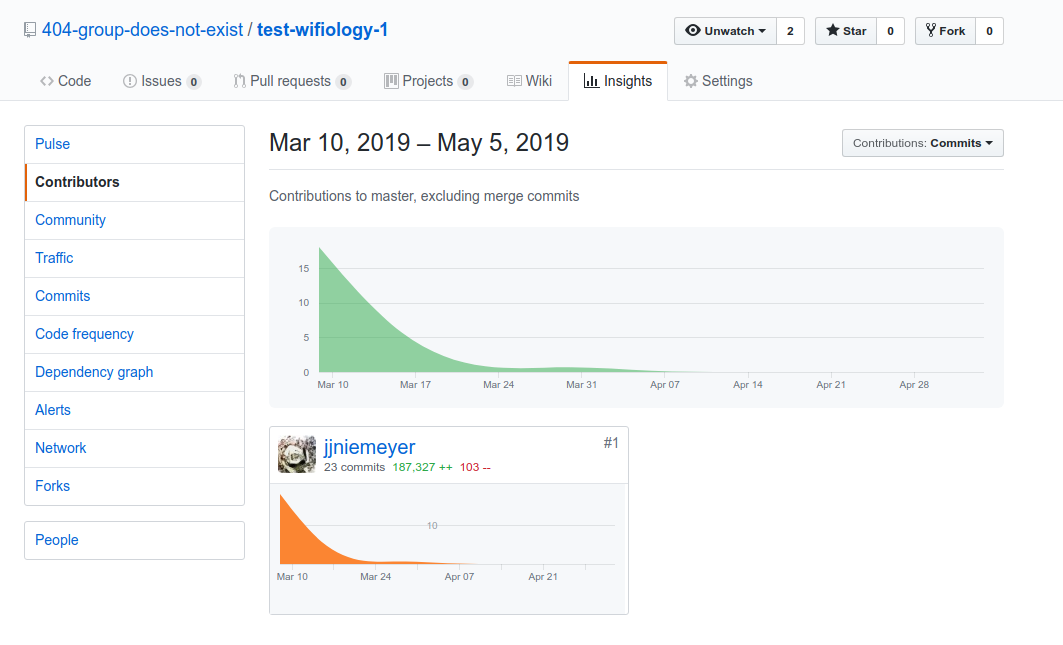
\includegraphics[width=1.0\textwidth]{testWifiologyContrib}
	\caption{Wifiology Test Repo. Contributions}
	\end{figure}
	
	\begin{figure}[h]
	\label{fig:selenium_tests_contrib}
	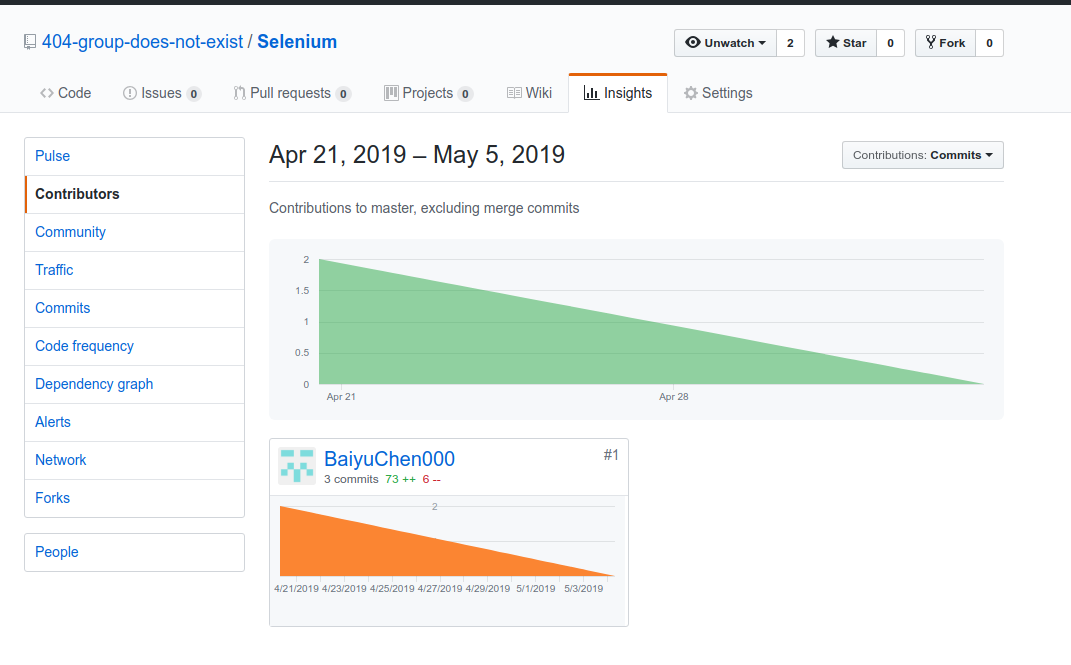
\includegraphics[width=1.0\textwidth]{seleniumTestsContrib}
	\caption{Selenium Tests Contributions}
	\end{figure}
	
	\begin{figure}[h]
	\label{fig:listener_node_contrib}
	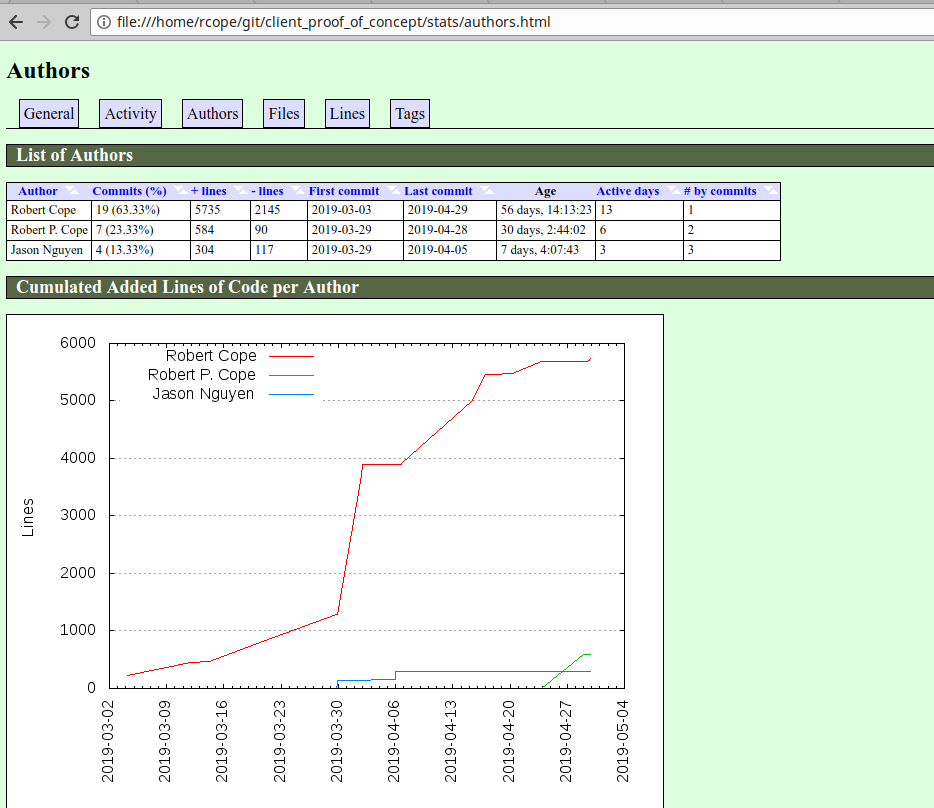
\includegraphics[width=1.0\textwidth]{listenerNodeContrib}
	\caption{Listener Node Contributions}
	\end{figure}
	
	\begin{figure}[h]
	\label{fig:core_server_contrib}
	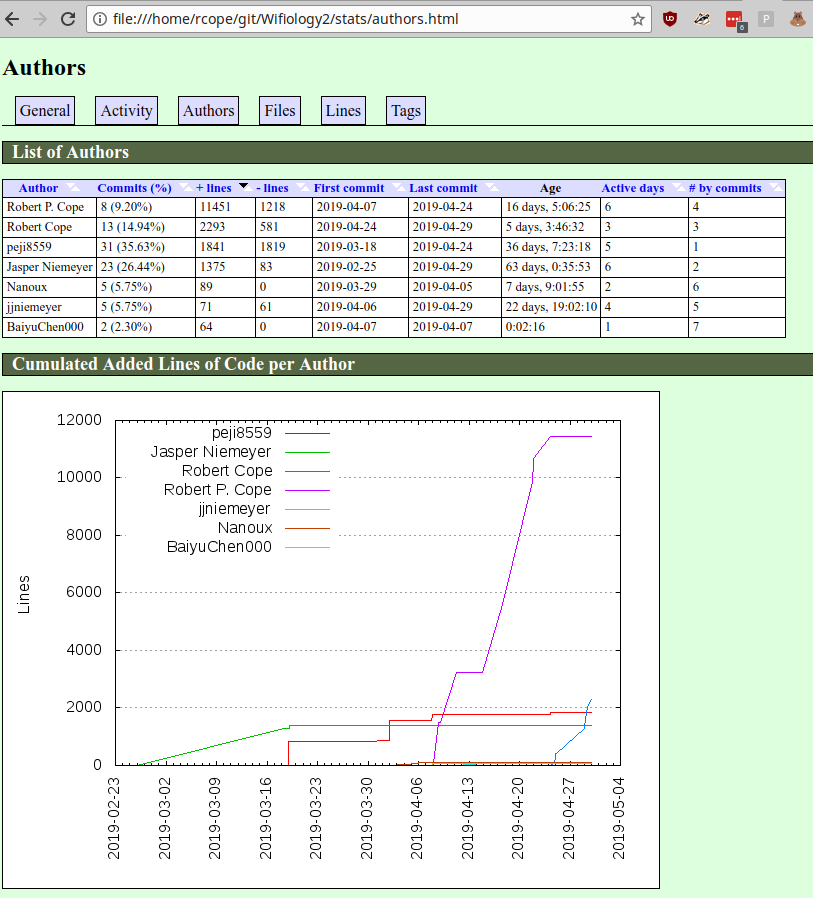
\includegraphics[width=1.0\textwidth]{coreServerContrib}
	\caption{Core Server Contributions}
	\end{figure}
	
	\begin{figure}[h]
	\label{fig:minutes_contrib}
	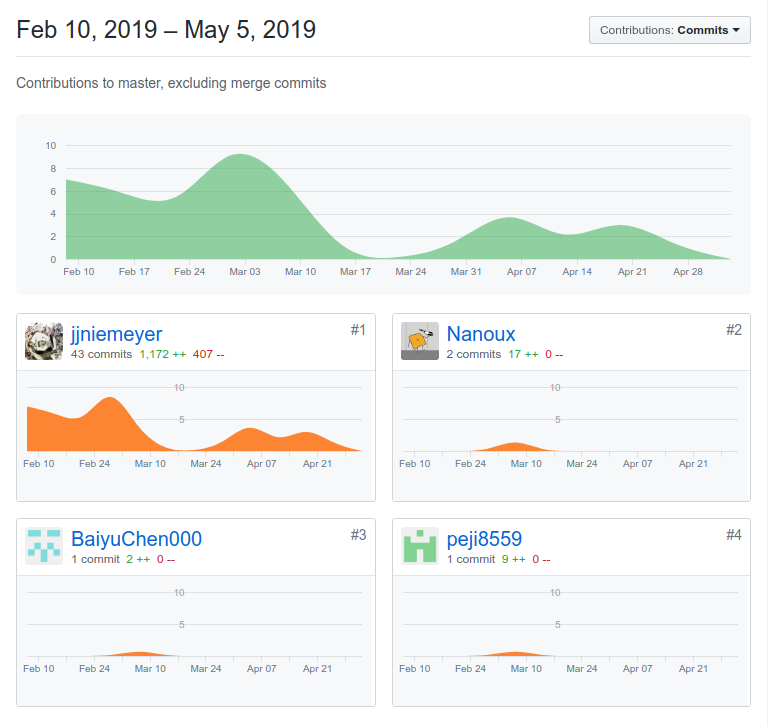
\includegraphics[width=1.0\textwidth]{minutesContrib}
	\caption{Minutes Contributions}
	\end{figure}
	
	\begin{figure}[h]
	\label{fig:milestones_contrib}
	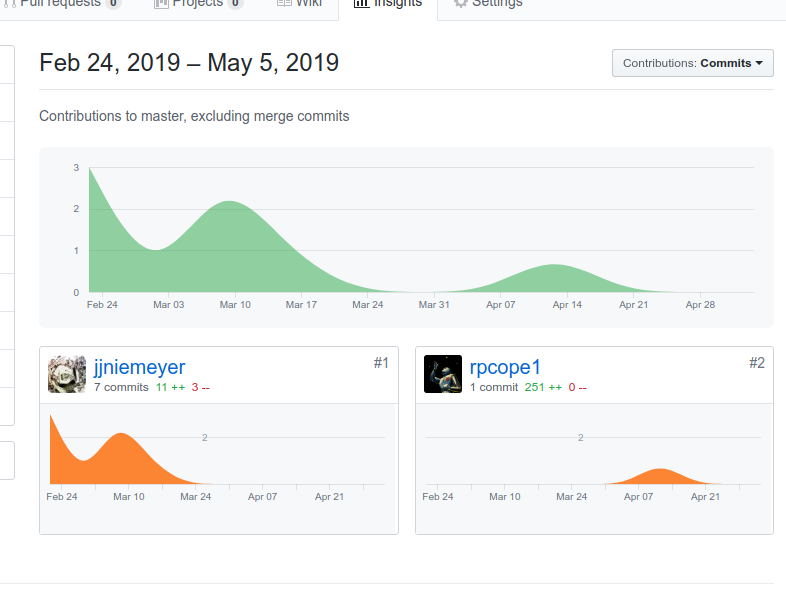
\includegraphics[width=1.0\textwidth]{milestonesContrib}
	\caption{Milestones Contributions}
	\end{figure}
	
	\subsection{Deployment}
	
	A running instance of the Wifiology app can be found at \href{https://wifiology.copesystems.com/}{https://wifiology.copesystems.com/}.
	As of the writing of this document, there is at least one listener node actively reporting back to the application instance, and 
	registration into the application is still turned on.
	
\end{document}